\chapter{背景}
\label{background}

本章では本研究の背景となる,論文とはなんなのか,およびその構成要素について述べる.

\section{論文とは}
\label{background:whtthesis}
論文とは,人類に新たな発見・知見をもたらす文書である.
既存の何か問題を解決する新たな発見があり,それの解法が正しいことを``論理的''に示す.
多くの場合,``査読''と呼ばれるプロセスを経て,著者以外に正当性を検証される\footnote{学会論文には査読を経ずに,投稿すれば発表ができ,学会論文集(Proceedings)に掲載されるものもある.} .
表~\ref{table:typepaper}に論文の大まかな分類を示す.
それぞれにおいて,英語で執筆され,全世界的に公開されるものを``国際論文'',日本語で執筆されるものを``国内論文''と呼ぶ.
本稿の想定読者\footnote{RGの学部生}は,少なくとも学位論文を書かなければ卒業することはできない.

\begin{table}[!hbtp]
    \begin{center}
        \caption{論文の分類}
				\label{table:typepaper}
  			\begin{tabular}{|l|l|}
					\hline
    			学位論文 & 学位(学士・修士・博士)を取得するための論文 \\
					\hline
    			ジャーナル(論文誌)論文 & 論文を掲載する雑誌に掲載される論文  \\
    			\hline
					学会論文 & 学会で発表するための論文 \\
    			\hline \hline
					プレプリント & ArXivなどで査読を経ずに公開される論文  \\
  				\hline
				\end{tabular}
		\end{center}
\end{table}

多くの学部生は論文を書いた経験はないと考えられ,そうした人はどのように論文を執筆したら良いのだろうか.
少なくとも学部生レベルで``人類に全く新しい知見''を切り開くのは困難である.
世界中では優秀な研究者たちが日進月歩で研究をしている.
その研究者たちが全く考えが及ばない内容を,一個人が突然発見することはほとんどないと言っていいだろう.

論文を書くにあたり,最も重要な最初のステップは,``論文を読むこと(サーベイ)''である.
先人たちがいくら素晴らしいシステムを考案していても,全ての問題が解決され,完璧なシステムを作ることは困難である\footnote{``銀の弾丸は存在しない''などと言われる.}.
後述するが,論文ではその論文で未解決な問題を列挙するような節を作る.
我々が最初のステップとして実施できることは,既存の論文を読み,今までの先人たちが解決できなかった問題を探ることである.

そうして見つかった問題に対して,少しでも解決方法が提示できれば,学部生としては上出来と言わざるを得ない.
むしろ,今までの世界中で行われている研究の流れに沿って,未解決な問題を解決できたのならば,それほど素晴らしいことはない.
こうして今までの研究の上に,自分の研究を行うことで新たな知見を開くことを``巨人の肩に立つ(nani gigantum umeris insidentes)''と言う.
自分がいきなり巨人になることは難しいが,巨人の肩に乗ればほんの少しだけ,巨人よりも上の世界を見ることができるのだ.

\section{論文を執筆するプロセス}
\label{background:process}

\subsection{サーベイの方法}
\label{backgorund:servey}
これまでに出ている論文を探し,自分が興味ある分野の最先端の研究と現状の課題を整理する作業を``サーベイ''と呼ぶ.
サーベイにおいては,むやみに論文を読むのではなく,その分野において重要な論文を見つけ出し,そこから派生する研究を紐解いていくことが重要である.
この作業によって,世界中でどんな研究がこれまでどんな経緯で行われてきたかということが明らかになっていく.
その上で,自分がどんな問題に対して,どんな解決策を提示し,それによってどのような良いことが生まれるのか(貢献),を整理していくことが研究に他ならない.

まず,論文を探すときはGoogle Scholer~\cite{googlescholer}などの論文検索サービスを利用するのが良いだろう~\footnote{その他探してきた論文をまとめるMendeley~\cite{mendeley}などの文献管理サービスを利用するとより今後捗るが,ここでは紹介のみに留める.}.
ひとまず自分の興味のある分野のキーワードを調べてみよう.
図~\ref{img:scholersearch}は``Bitcoin''で検索した結果である.
デフォルトではキーワードに対して関連性の高い論文順に並んでいる.

\begin{figure}[htb]
    \begin{center}
        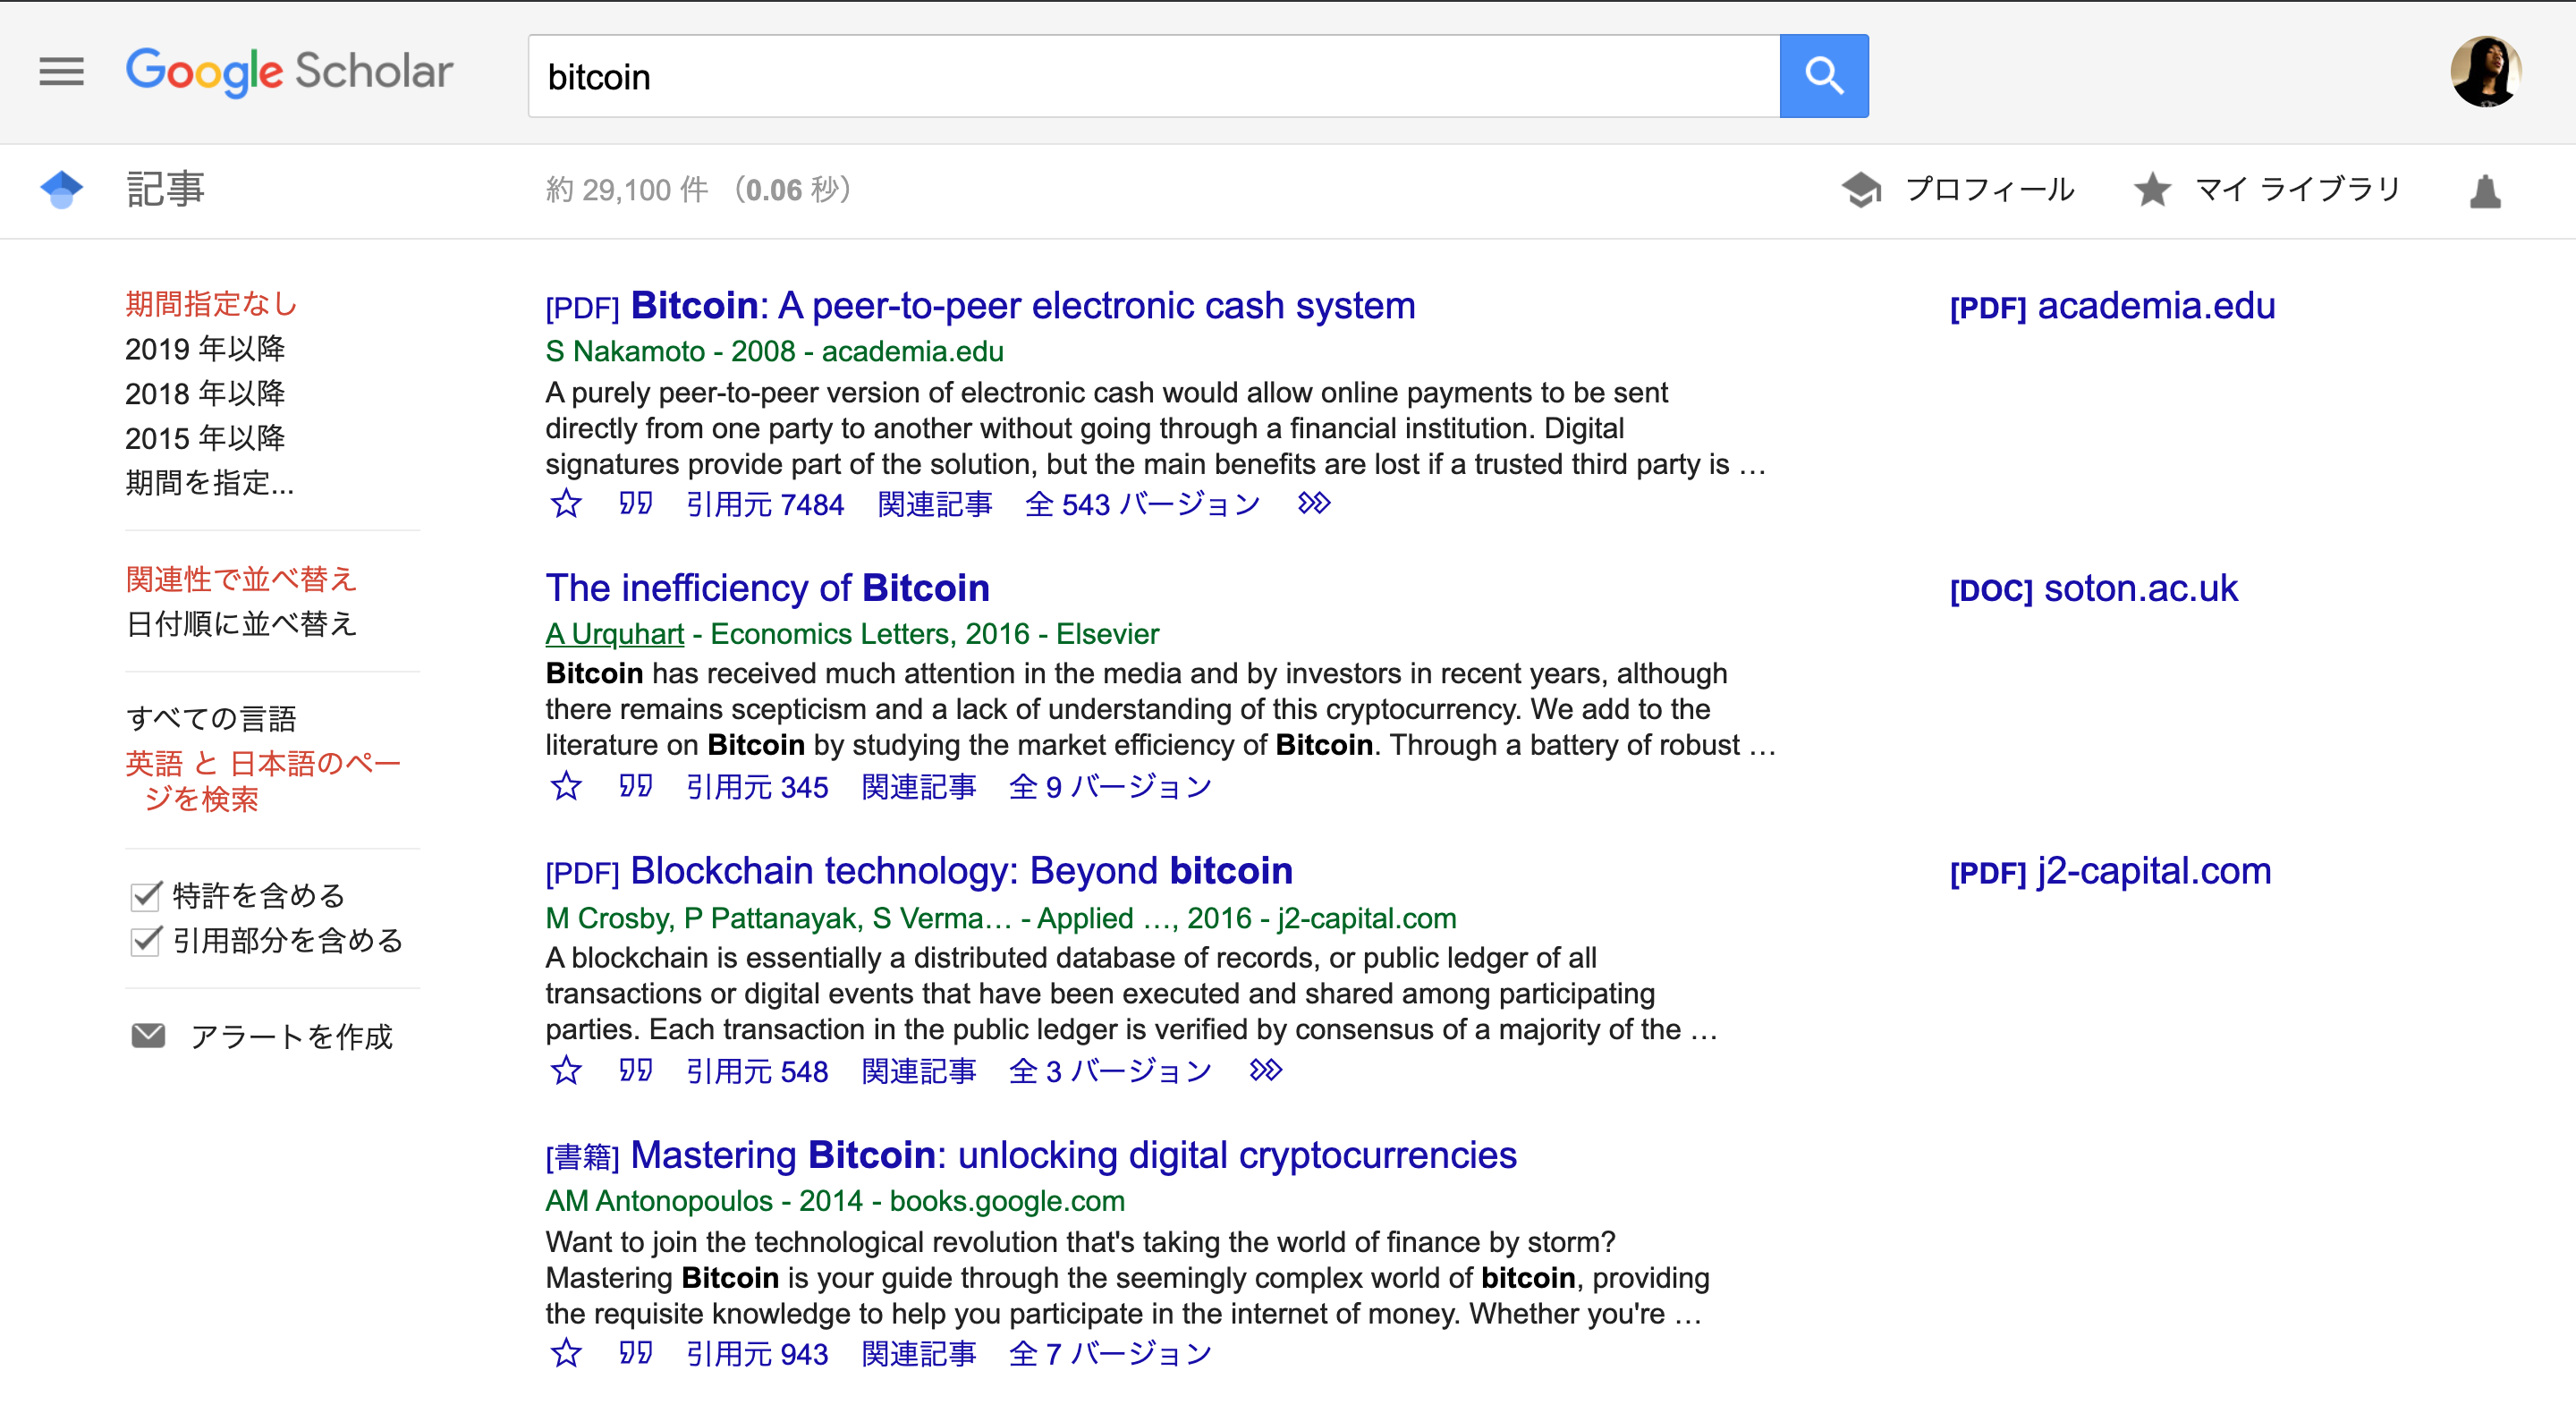
\includegraphics[width=450pt]{./img/scholersearch.png}
        \caption{Google Scholer検索結果画面}
        \label{img:scholersearch}
    \end{center}
\end{figure}

どの論文を読むべきかの一つの指標となるのが,被引用数である.
~\ref{background:whtthesis}節で述べたように,多くの論文は既存の論文を``引用''し,新規の貢献を述べている.
ここで,多くの論文に引用されるということは,その論文は``比較的''多くの研究がその上で実施できるレベルの,その分野を切り開いた論文である可能性が高い.
図~\ref{img:scholersearch}でも,Bitcoinの最初の設計文書である``Bitcoin: A peer-to-peer electronic cash system''が比較的高い引用数を示している.
一方で,被引用数が高くても,必ずしも論文としての質が高いとは限らない場合もある.
被引用数は一つの指標であり,傾向を示すものでしかないことに注意するべきである.


また,被引用数が高いだけでなく当然内容についても精査しなければならない.
その場合は,タイトルを眺め,興味のありそうなものをとりあえず読むのが良いだろう.
しかし,ここでいきなり論文の本文を読んではいけない.
論文には必ず``概要(abstract)''の節が存在し,その論文の要約が掲載されている.
要約を読み,中身を把握できたら初めて論文本文を読むことになる.

\subsection{論文の読み方}
\label{background:readpaper}


\section{論文の構成}
\label{background:structure}


\if0
\begin{figure}[h]
    \begin{center}
        \includegraphics[scale=0.4]{./img/hashrate.png}
        \caption{2017年1月のハッシュレート分布 出典:Blockchain.info\cite{bitcoinhashrate}}
        \label{img:hashrate}
    \end{center}
\end{figure}
\fi
